\documentclass{beamer}

% Setup appearance:

%\usetheme{Darmstadt}
%\usetheme{Warsaw}
%\usetheme{Boadilla}
%\usetheme{Hannover}   %jó
%\usetheme{Marburg}      %jó
%\usetheme{Singapore}  %jó
%\usetheme{Szeged}
\usetheme{CambridgeUS}

%color theme
\usecolortheme{beaver}
%\usecolortheme{reen}


\usepackage[magyar]{babel}
%\usepackage[english]{babel}

\usepackage[utf8]{inputenc}
\usepackage{times}
\usepackage[T1]{fontenc}

\usepackage{amsmath}
\usepackage{graphicx}
\usepackage{enumerate}

\usepackage{caption}
%\usepackage{subcaption}

\usepackage{epstopdf}

\usepackage{color}
\usepackage{listings}
\definecolor{javared}{rgb}{0.6,0,0} % for strings
\definecolor{javagreen}{rgb}{0.25,0.5,0.35} % comments
\definecolor{javapurple}{rgb}{0.5,0,0.35} % keywords
\definecolor{javadocblue}{rgb}{0.25,0.35,0.75} % javadoc
 
\definecolor{dkgreen}{rgb}{0,.6,0}
\definecolor{dkblue}{rgb}{0,0,.6}
\definecolor{dkyellow}{cmyk}{0,0,.8,.3}

\lstset{
  language        = php,
  basicstyle      = \small\ttfamily,
  keywordstyle    = \color{dkblue},
  stringstyle     = \color{red},
  identifierstyle = \color{dkgreen},
  commentstyle    = \color{gray},
  emph            =[1]{php},
  emphstyle       =[1]\color{black},
  emph            =[2]{if,and,or,else},
  emphstyle       =[2]\color{dkyellow}}
 
%\lstset{language=Java,
%basicstyle=\ttfamily,
%keywordstyle=\color{javapurple}\bfseries,
%stringstyle=\color{javared},
%commentstyle=\color{javagreen},
%morecomment=[s][\color{javadocblue}]{/**}{*/},
%numbers=left,
%numberstyle=\tiny\color{black},
%stepnumber=2,
%numbersep=10pt,
%tabsize=4,
%showspaces=false,
%showstringspaces=false}
%\lstset{
%language=HTML,
%basicstyle=\ttfamily,
%keywordstyle=\color{blue},
%breaklines=true, 
%commentstyle=\color{javagreen},
%numbers=left,
%numberstyle=\tiny\color{gray},
%stepnumber=2,
%numbersep=5pt,
%}


\definecolor{okgreen}{rgb}{0,1,0}
\definecolor{wrongred}{rgb}{1,0,0}

\newcommand{\OK}{{\color{okgreen}\checkmark}}
\newcommand{\WRONG}{{\color{wrongred}X}}
\newcommand{\QUESTION}[1]{{\color{wrongred}¿} #1 {\color{wrongred}?}}
\newcommand{\QUESTIONMARK}{{\color{wrongred}?}}
\newcommand*{\supervisor}[1]{\def\supname{#1}}

% Author, Title, etc.

\title[Android Fejlesztés]{Szoftverfejlesztés Android platformra}

\author{Adam Satan}

\institute{Minőségbiztosítás informatikája}

\date{\the\year}

\begin{document}

\maketitle
%\begin{frame}
%  \titlepage
%\end{frame}

\section{Bevezető}

\begin{frame}[fragile]{Android}
	\begin{minipage}{0.49\textwidth}		
		\begin{itemize}
			\item Google - Android
			\item Android Studio
			\item Fejleszési nyelvek
			\item Szoftver fejlesztés
			\item Szoftver tesztelés	
		\end{itemize}
	\end{minipage}
	\begin{minipage}{0.49\textwidth}
		
\includegraphics[width=1 \linewidth]{figures/android.png}
	\end{minipage}
\end{frame}
\begin{frame}[fragile]{Google LCC}
	\begin{minipage}{0.49\textwidth}
		\begin{itemize}
				\item 19 éve alapították
				\item Fő bevételforrása: reklámok
				\item kb 73000 alkalmazott
				\item 767 Milliárd dolláros piaci érték
				\item Magyarország GDP-je: 120 Milliárd dollár 
		\end{itemize}
	\end{minipage}
\begin{minipage}{0.49\textwidth}
	\begin{itemize}
		\item Ismertebb munkásságai:
		\begin{itemize}
			\item Google kereső
			\item Gmail
			\item Chrome
			\item Fiber
			\item Maps
			\item Docs, Drive
			\item Chromebook
			\item Android
		\end{itemize}
	\end{itemize}
\end{minipage}
\end{frame}
\begin{frame}[fragile]{Google}
	\begin{minipage}{0.8\textwidth}
		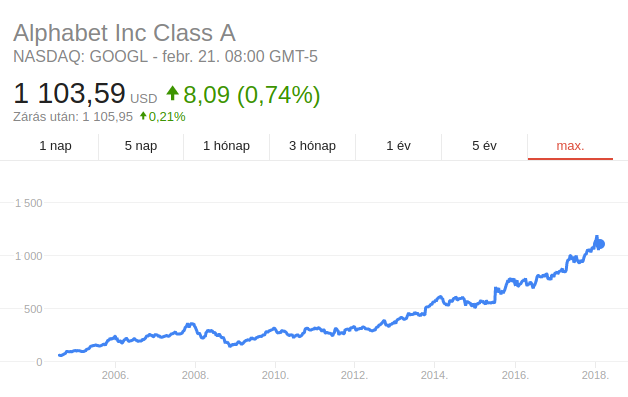
\includegraphics[width=1 \linewidth]{figures/share.png}
	\end{minipage}
\end{frame}
\begin{frame}[fragile]{Android}
	\begin{minipage}{0.49\textwidth}
		\begin{itemize}
			\item 2008 szeptember
			\item Linux alapú mobil operációs rendszer
			\item ARM, x86, x64
			\item Telefon, Tablet, Okosóra, TV, Autó
		\end{itemize}
	\end{minipage}
	\begin{minipage}{.49\textwidth}
		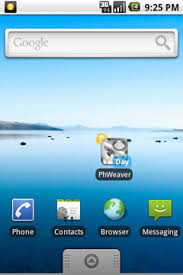
\includegraphics[width=.8\linewidth]{figures/android10.jpeg}
	\end{minipage}
\end{frame}
\begin{frame}[fragile]{Android}
	\begin{minipage}{0.49\textwidth}
		\begin{itemize}
			\item 8. verzió (2017 December)
			\item 432 millió okostelefonból 352 millió androidos (87\%)
			\item 3,638,448 alkalmazás (2018 febr 20)
			\item Átlagosan havonta 60,000 új app
		\end{itemize}
	\end{minipage}
	\begin{minipage}{.49\textwidth}
		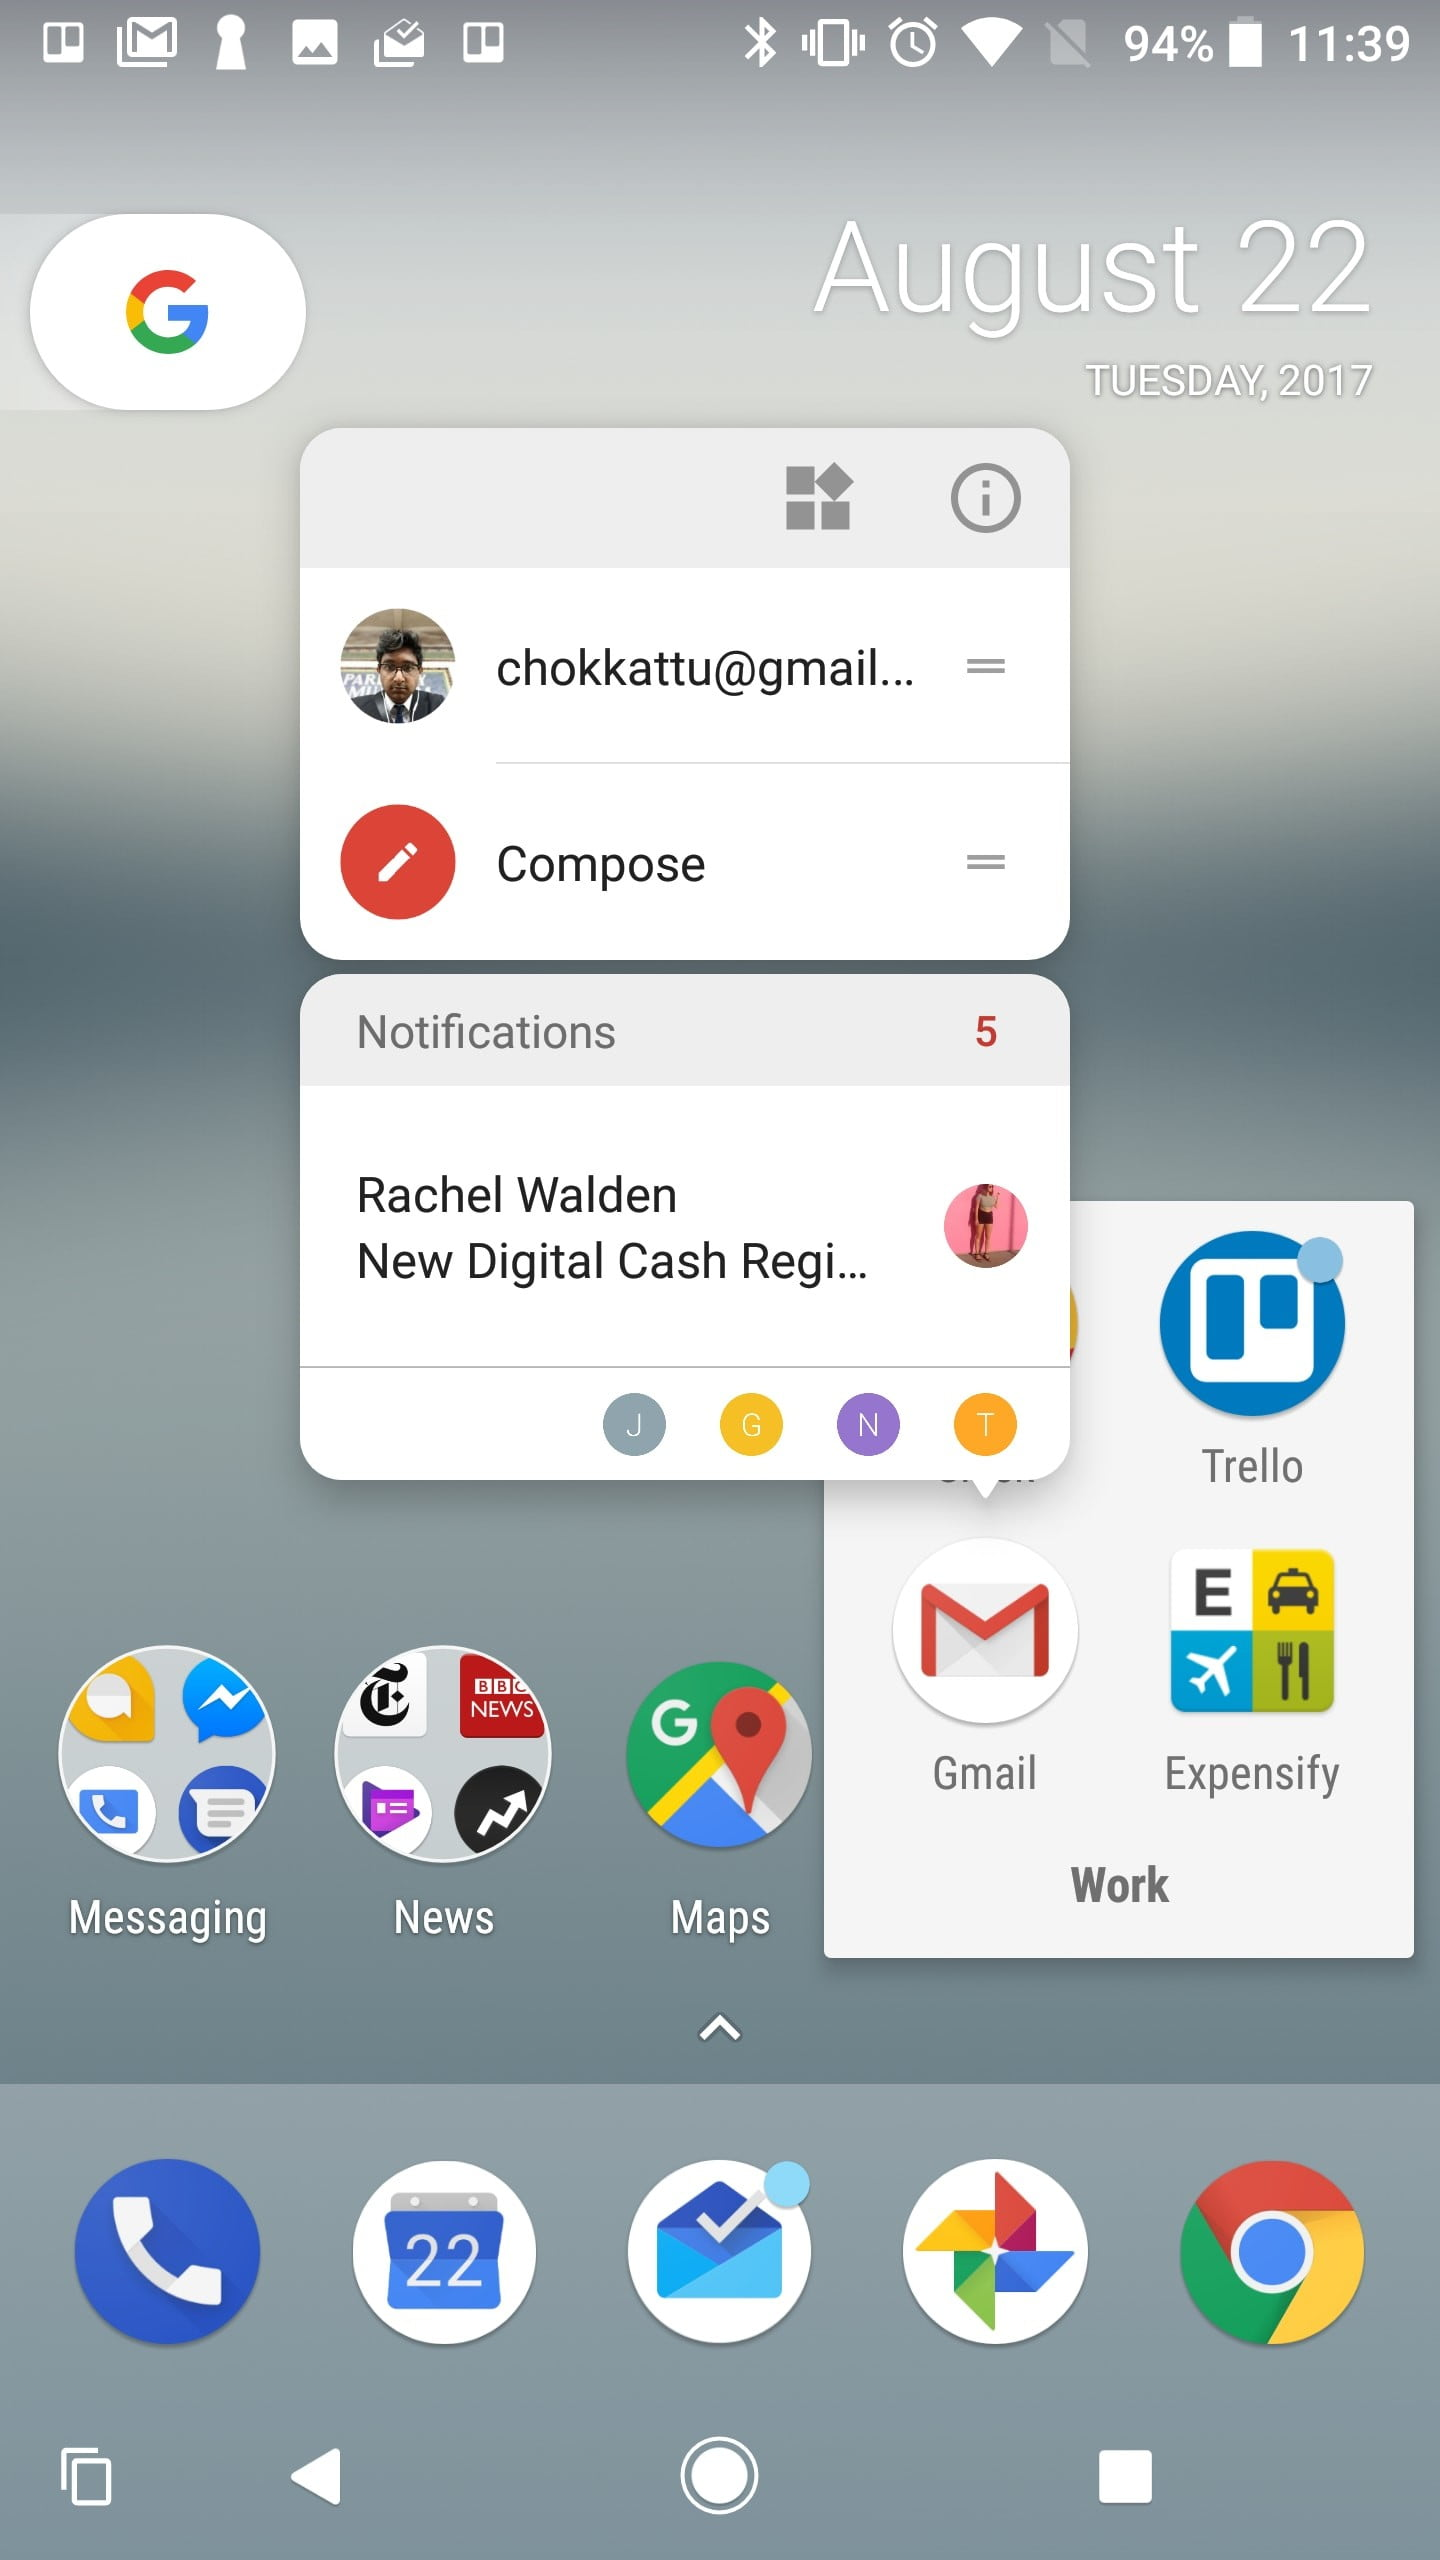
\includegraphics[width=.8\linewidth]{figures/android80.jpg}
	\end{minipage}
\end{frame}
\begin{frame}[fragile]{Android fejlesztő}
	\begin{minipage}{0.49\textwidth}
		\begin{itemize}
			\item 80000\$ átlagfizetés
			\item 1,000,000 reklámos alkalmazás
			\item 432 millió okostelefonból 352 millió androidos (87\%)
			\item 3,638,448 alkalmazás (2018 febr 20)
			\item Átlagosan havonta 60,000 új app
		\end{itemize}
	\end{minipage}
	\begin{minipage}{.49\textwidth}
		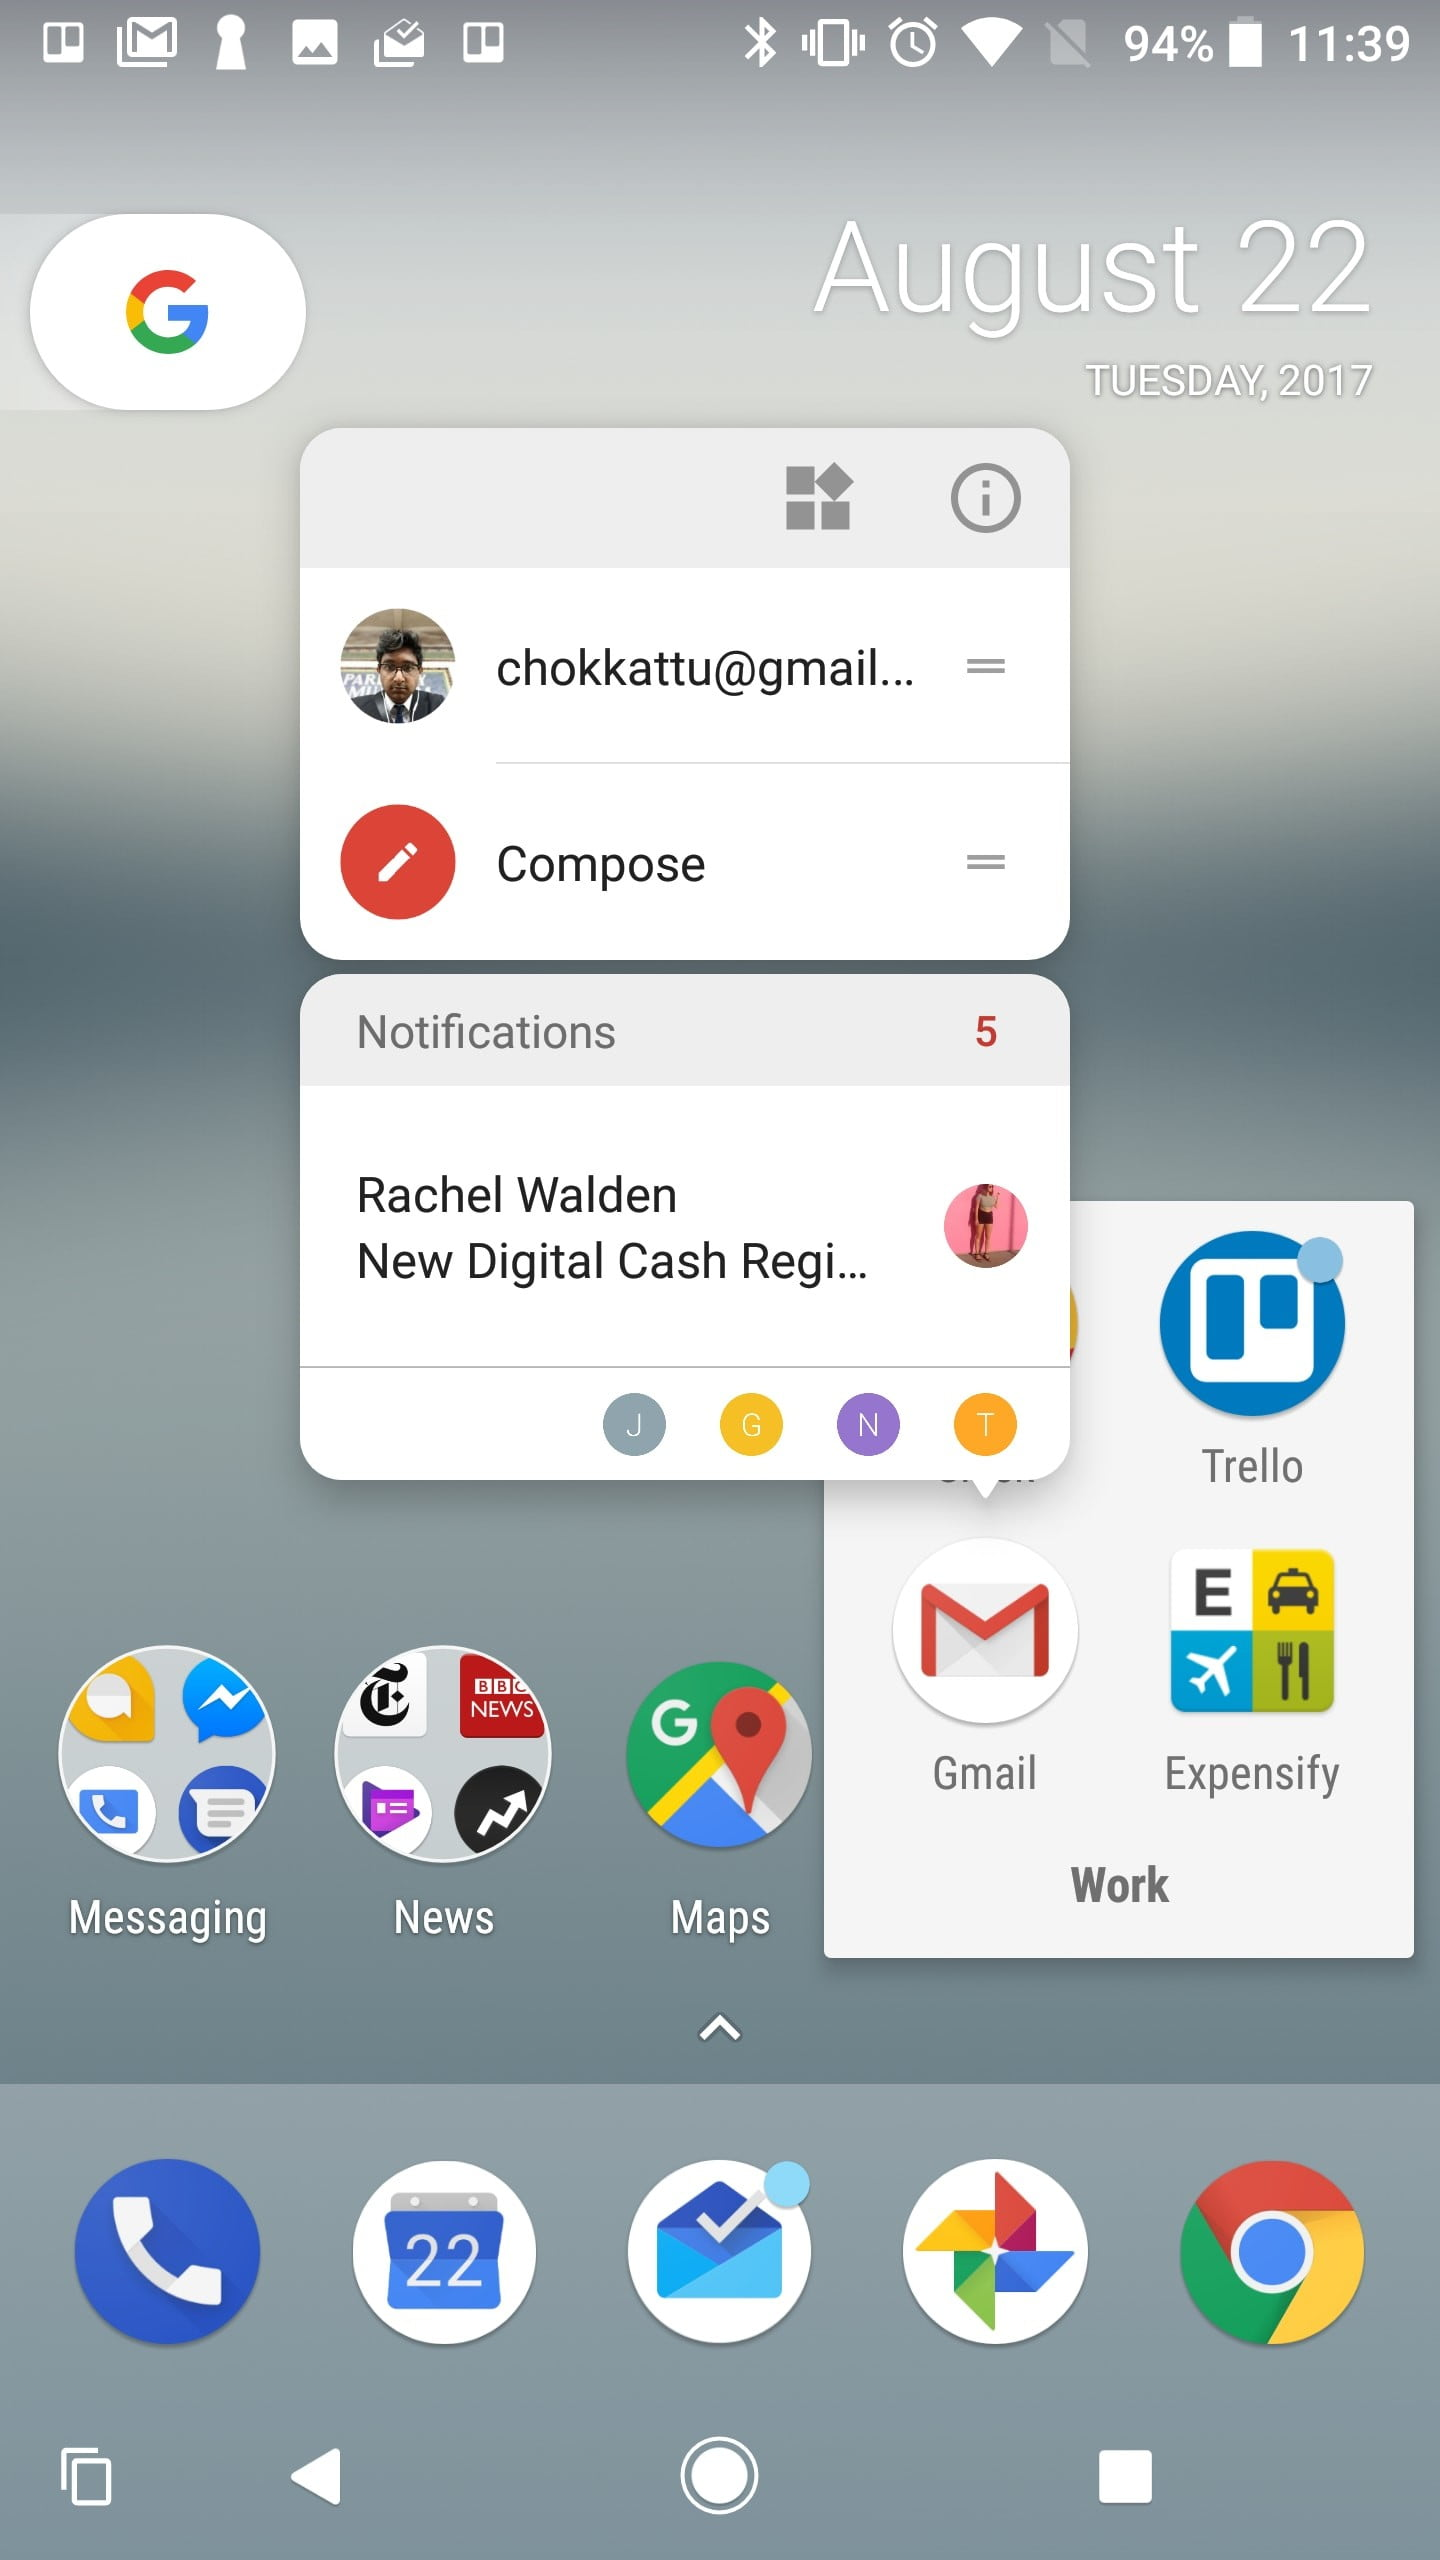
\includegraphics[width=.8\linewidth]{figures/android80.jpg}
	\end{minipage}
\end{frame}
\section{}

\begin{frame}
\centering
\LARGE Thank you for your attention!
\end{frame}

\end{document} 